% ======================= 5. MODELACIÓN =======================
\section{Modelación y validación}\label{sec:modelacion}

\subsection{Ruta de análisis}\label{sec:ruta}
La Tabla~\ref{tbl:ruta} vincula cada técnica con su pregunta, sus variables, su respaldo metodológico y artículos que la aplicaron en contextos ambientales o con series de tiempo. Para nuestro objetivo, el PCA muestra qué condiciones meteorológicas varían juntas. El LDA, fijado en el protocolo, mide cuánto separa la meteorología los días con y sin superación por encima de estación y temporada. La logística responde lo mismo sin suponer normalidad y expresa cada efecto en momios. El bootstrap por bloques da un intervalo que respeta la persistencia entre días y estaciones. La validación progresiva comprueba que la mejora se repite en años que el modelo no vio.

\begin{table}[!htbp]
\centering\footnotesize
\caption{Ruta de análisis: técnica y tipo, pregunta, variables, justificación, respaldo metodológico y aplicación previa en contextos ambientales o de series de tiempo.}
\label{tbl:ruta}
\begin{tabularx}{\textwidth}{>{\raggedright\arraybackslash}p{2.3cm}>{\raggedright\arraybackslash}p{2.5cm}>{\raggedright\arraybackslash}p{2.2cm}L>{\raggedright\arraybackslash}p{2.0cm}L}
\toprule
Técnica & Pregunta & Variables & Por qué es adecuada & Respaldo & Aplicación previa\\
\midrule
Componentes principales (PCA; interdependencia) & ¿Cómo se estructura la correlación de la meteorología? & 8 meteorológicas, como anomalías por estación & Resume variables correlacionadas en pocos ejes; describe, no predice & Jolliffe y Cadima (2016) & Ramírez-Velarde et al. (2024): meteorología de la ZMM y contingencias; Mohd Shafi'i y Juahir (2024): 8 estaciones de Malasia\\
LDA (dependencia, fijada en el protocolo) & ¿Cuánto mejora M1 a M0? & Estación y temporada; en M1, + 8 meteorológicas & Función lineal interpretable; con la misma partición, M1 − M0 se atribuye a la meteorología & Johnson y Wichern (2007); Krzanowski (1975) & Mohd Shafi'i y Juahir (2024): 90.5\,\% de los casos bien asignados a grupos de estaciones por contaminación\\
Regresión logística (dependencia, en paralelo) & ¿Qué variables influyen? ¿Depende la conclusión de los supuestos del LDA? & Las mismas que el LDA & No supone normalidad ni covarianzas iguales; referencia para interpretar las variables & Efron (1975); James et al. (2021) & Vélez-Pereira et al. (2025): superaciones diarias de PM2.5 y PM10 en Chile; Saminathan y Malathy (2023): PM2.5 con meteorología en Pekín\\
Bootstrap pareado por bloques & ¿Qué tan incierta es la \dauc? & Predicciones de la prueba en bloques de 14 días & La contaminación alta persiste días y afecta a varias estaciones & Carlstein (1986); Künsch (1989) & Wilks (2019): datos atmosféricos autocorrelacionados\\
Validación temporal progresiva & ¿Se sostiene la mejora en años posteriores? & Entrenar en años anteriores y evaluar el siguiente & Con datos ordenados en el tiempo, la validación aleatoria sobreestima el desempeño & Roberts et al. (2017) & Roberts et al. (2017): datos ecológicos con estructura temporal\\
\bottomrule
\end{tabularx}
\end{table}

\subsection{Componentes principales}\label{sec:pca-metodo}
El PCA se ajustó solo con el entrenamiento, sobre las anomalías de cada variable respecto de la media de su estación, para que los ejes describan la variación meteorológica y no las diferencias entre sitios. La adecuación es modesta: KMO = 0.64, valor que Kaiser y Rice (1974) clasifican como mediocre; por ello el PCA se utiliza con fines exploratorios. La prueba de Bartlett (1950) rechaza la esfericidad (χ² = 26\,503, gl = 28, p < 0.001). Tres valores propios superan 1 (criterio de Kaiser, 1960) y explican el 66.5\,\% de la varianza. \textbf{Ese 66.5\,\% es la parte de la variación conjunta de las ocho variables meteorológicas que resumen los tres ejes; no significa que la meteorología explique el 66.5\,\% de las superaciones.} Tampoco es un predictor: maximizar la varianza no maximiza la separación entre clases, y su primer eje mezcla variables que se asocian con la superación en sentidos contrarios (Sección~\ref{sec:coef}). En la etapa 3, usar los tres componentes en lugar de las ocho variables dio una mejora menor (Anexo~A). \textbf{El PCA resume la correlación entre variables, pero no elimina la autocorrelación temporal de los días.}

\subsection{LDA y el tratamiento de estación y temporada}\label{sec:lda}
\textbf{Codificación.} Estación (13 niveles) y temporada (3) entran como variables indicadoras, \emph{k} − 1 por factor, con categoría de referencia CE (Obispado) y temporada cálida-húmeda: 12 indicadoras de estación y 2 de temporada, estandarizadas con el entrenamiento como el resto de los predictores. \textbf{M0} usa solo esas 14 indicadoras. Su función discriminante asigna a cada día un puntaje que es la suma de un efecto de estación y uno de temporada, así que M0 da una misma probabilidad a todos los días de cada una de las 39 combinaciones estación × temporada: es la referencia de lo que ya se sabe sin la meteorología diaria. \textbf{M1} agrega a las mismas indicadoras las ocho variables meteorológicas continuas (22 predictores).

\textbf{Por qué es apropiado para los dos modelos.}
\begin{enumerate}
\item Mismo método y misma partición: la diferencia M1 − M0 se atribuye a la meteorología y no al clasificador.
\item El criterio de Fisher, que busca la combinación lineal que separa las medias de las clases en relación con la dispersión dentro de ellas, no requiere normalidad. La regla y sus probabilidades solo son óptimas si los predictores son normales con una covarianza común en las dos clases (Johnson \& Wichern, 2007).
\item Con indicadoras, la normalidad multivariada no se cumple literalmente. Por eso el LDA se usa como clasificador lineal y no como modelo generativo bien especificado. Para predictores mixtos, Krzanowski (1975) propuso el modelo de localización, que generaliza el discriminante a variables binarias y continuas; la regla lineal que usamos es una aproximación que supone que el efecto de la meteorología sobre la separación es el mismo en todas las estaciones y temporadas.
\item El logit de la probabilidad posterior del LDA es lineal en los predictores, igual que en la regresión logística. Con normalidad condicional y covarianza común, el LDA puede ser más eficiente asintóticamente que la logística (Efron, 1975). La logística no exige una distribución normal de los predictores, aunque sí especifica una forma para la probabilidad condicional; su comparación con el LDA aporta aquí evidencia empírica de estabilidad.
\end{enumerate}

\textbf{Dos clasificadores en paralelo.} Conservamos el LDA, fijado en el protocolo antes de evaluar, y reportamos junto a él la regresión logística con los mismos predictores, que da resultados similares y es la referencia para interpretar las variables (Sección~\ref{sec:logistica}). Tampoco resuelve todo: requiere especificar bien la relación de cada predictor con el logit (razón 4), y la autocorrelación invalida su inferencia convencional.

\textbf{Prior y corte.} La probabilidad previa es la prevalencia del entrenamiento (0.259), y un día se clasifica como superación si su probabilidad posterior es al menos esa prevalencia. El corte se fijó antes de ver la prueba; la Sección~\ref{sec:umbral} evalúa cortes elegidos con el entrenamiento para usos concretos.

\subsection{Supuestos: qué se revisó, qué implica y qué no se puede concluir}\label{sec:supuestos}

\begin{table}[!htbp]
\centering\footnotesize
\caption{Supuestos del LDA y un diagnóstico adicional de los residuos, revisados en el entrenamiento (n = 10\,965) y en los errores de la prueba (n = 6\,863), con su implicación y su tratamiento (base v2).}
\label{tbl:supuestos}
\begin{tabularx}{\textwidth}{>{\raggedright\arraybackslash}p{2.45cm}>{\raggedright\arraybackslash}p{2.7cm}LLL}
\toprule
Supuesto & Diagnóstico & Resultado & Implicación & Cómo se tomó en cuenta\\
\midrule
Normalidad multivariada por clase & Mardia (1970), 8 meteorológicas; las indicadoras son discretas & No se cumple: asimetría χ² = 99\,015 y 198\,072 (gl = 120, p < 0.001); lluvia con asimetría de 7.6 y 19.9 & No está garantizada la optimalidad de la regla ni la calibración de sus probabilidades & LDA como clasificador; logística como contraste (0.071)\\
Igualdad de covarianzas & M de Box (1949) y razón de desviaciones por clase & No se cumple: χ² = 3\,213 (gl = 36, p < 0.001); diferencia sobre todo en la lluvia (razón 0.40) y en \emph{v} (0.78); en las demás, 0.85–1.05 & La igualdad de covarianzas no está respaldada; una frontera lineal puede perder eficiencia & QDA como alternativa: no mejora (0.788 frente a 0.792)\\
Independencia & ACF del residuo dentro de cada estación; correlación entre estaciones el mismo día & No se cumple: ACF a 1 día de 0.42 en el residuo de M1 (0.50 en la respuesta); 0.36 entre estaciones & Los errores estándar usuales no valen & Bootstrap por bloques; estabilidad por bootstrap; sin valores p\\
Multicolinealidad & VIF y número de condición & Baja: VIF máximo 2.28 (temperatura); número de condición 2.97 & Los coeficientes se pueden leer en conjunto & Presión como anomalía; interpretación conjunta\\
Diagnóstico adicional: variación de los residuos y calibración & Varianza de Y − \^{p} por temporada y estación (Brown-Forsythe, solo descriptivo por la dependencia); error por decil & La varianza de Y − \^{p} cambia entre temporadas (0.086–0.205; F = 503); en el decil más alto el error es 1.34 veces el esperado; pendiente de recalibración de 0.82 & Esperable en parte por la respuesta binaria; no es un supuesto incumplido del LDA & Las probabilidades necesitan recalibración antes de comunicarse como riesgos; se usan como puntajes\\
\bottomrule
\end{tabularx}
\end{table}

La Tabla~\ref{tbl:supuestos} muestra que el LDA no cumple sus supuestos distribucionales, y conviene precisar qué hace cada herramienta. El bootstrap por bloques estima la incertidumbre del \textbf{desempeño} respetando grupos de fechas, pero no vuelve independientes los datos con los que se ajusta el LDA: por eso no reportamos valores p de los coeficientes. El PCA controla la correlación entre variables, no la autocorrelación. La validación temporal mide cómo clasifica el modelo en años posteriores, aunque 2024–2025 ya se habían usado en una prueba de viabilidad preliminar (4 de octubre), en la evaluación de la etapa 3 y en la de la etapa 4. En las etapas 3 y 4 las decisiones se cerraron antes de evaluar la prueba con la base correspondiente; sin embargo, los cambios de la etapa 4 se decidieron después de conocer el resultado de la etapa 3. La mejora coincide con la de la validación progresiva dentro del entrenamiento (Sección~\ref{sec:validacion}), pero esa prueba ya no es completamente nueva y lo declaramos. Por todo esto, la evidencia que presentamos es empírica: validación temporal, comparación con la logística y estabilidad de los coeficientes. No interpretamos la función discriminante como un modelo generativo.

\subsection{Regresión logística: variables y linealidad}\label{sec:logistica}
\textbf{Variables relevantes.} Ajustamos M1 logístico con los 22 predictores estandarizados del LDA, con intervalos del mismo bootstrap por bloques del entrenamiento y sin valores p, que la dependencia entre días invalida. Las ocho meteorológicas tienen el signo del LDA (Figura~\ref{fig:coef}, panel b). Con lo demás constante, 1 DE más de rapidez del viento (0.85\,m/s) multiplica las momios de superación por 0.49 (IC 95\,\% [0.39, 0.62]); de presión respecto de lo normal del sitio (3.5\,mm\,Hg), por 0.58 [0.49, 0.70]; de temperatura (6.3\,°C), por 1.78 [1.24, 2.71]; de horas de lluvia (1.1\,h), por 0.81 [0.64, 0.93], y de radiación (0.08\,kW/m²), por 0.82 [0.67, 1.00], cuyo intervalo llega a 1, así que su efecto es débil. La humedad, \emph{u} y \emph{v} no tienen signo estable. Al permutar cada grupo de variables en la prueba, el AUC cae sobre todo con la temporada (0.138) y la estación (0.067); entre las meteorológicas, la caída se concentra en la presión, la rapidez del viento y la temperatura (0.03 a 0.05 cada una), y las demás lo mueven menos de 0.01. Como esas tres variables están correlacionadas, la permutación no permite ordenarlas entre sí: \textbf{la mejora de M1 descansa en el grupo ventilación–presión–temperatura}, con los dos clasificadores.

\textbf{Linealidad en la escala logit (Figura~\ref{fig:linealidad}, Anexo~C).} En el entrenamiento, los logits empíricos por deciles, ajustados por las demás variables, y un modelo aditivo generalizado (GAM) logístico con un spline penalizado por variable (Wood, 2017) muestran curvatura: de 5.4 a 8.4 grados de libertad efectivos, salvo en la lluvia (1.6); con días autocorrelacionados, esos grados de libertad pueden estar inflados. El efecto de la temperatura crece más rápido arriba de 28\,°C, el de la rapidez del viento se aplana arriba de 3\,m/s y el de la humedad cae arriba de 70\,\%; la presión es casi lineal. La regla fijada antes de evaluar la prueba (splines si suben el AUC de validación en ≥ 0.005 en los dos pliegues) se cumplió (+0.006 en 2022 y +0.021 en 2023), así que los reportamos como tratamiento de la no linealidad: en la prueba, M1 con splines llega a un AUC de 0.811 y mejora a M0 logístico en 0.090 [0.060, 0.120], frente a 0.071 con la forma lineal. El modelo principal no cambia; su forma lineal, si acaso, subestima lo que aporta la meteorología. La indicadora «llovió» no agrega nada a las horas de lluvia.

\subsection{Análisis de los errores}\label{sec:errores}
Con las predicciones de la prueba calculamos el residuo de cada día (superación observada menos probabilidad) y su autocorrelación dentro de cada estación (Figura~\ref{fig:acf}).

\begin{figure}[!htbp]
\centering
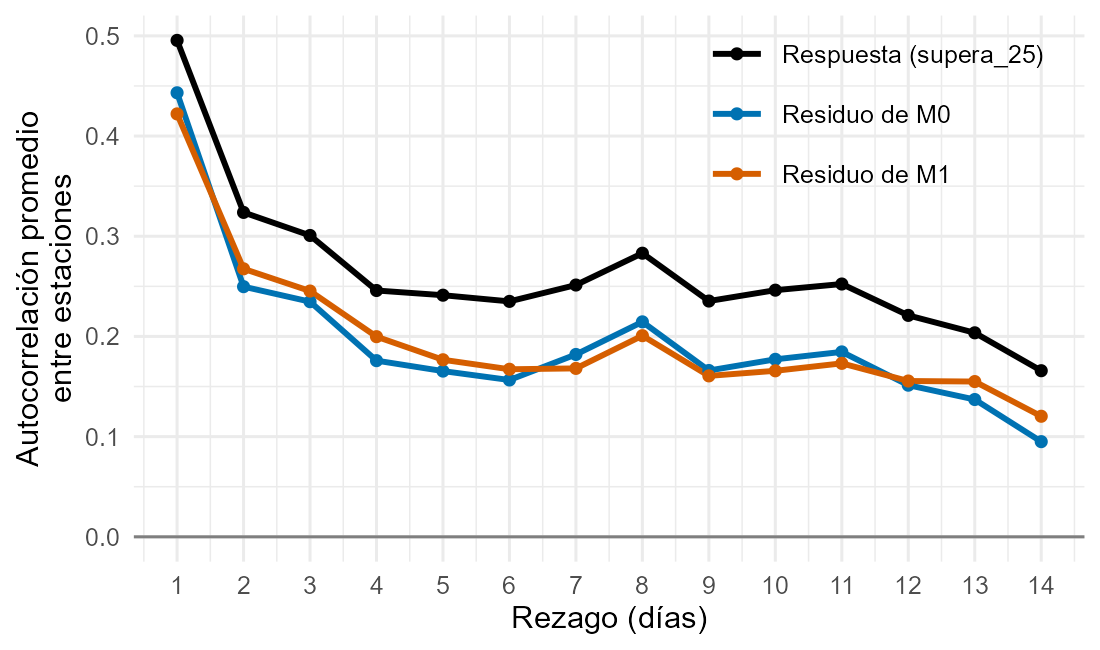
\includegraphics[width=0.46\textwidth]{figuras/acf_residuos_informe.png}
\caption{Autocorrelación promedio entre estaciones de la respuesta y de los residuos de M0 y M1, a rezagos de 1 a 14 días, dentro de cada estación (prueba 2024–2025, n = 6\,863).}
\label{fig:acf}
\end{figure}

La Figura~\ref{fig:acf} muestra que agregar la meteorología reduce poco la dependencia. La autocorrelación a un día baja de 0.50 en la respuesta a 0.44 con M0 y a 0.42 con M1, y la correlación entre estaciones el mismo día baja de 0.48 a 0.36. \textbf{El modelo no absorbe toda la dependencia}, y esa es la razón del bootstrap por bloques y del límite a la interpretación. La varianza de los errores también difiere entre temporadas y estaciones, algo esperable en parte con una respuesta binaria, y la calibración es imperfecta: la pendiente de la recalibración es 0.82, cuando el ideal es 1, y en todas las temporadas queda entre 0.69 y 0.76 (Anexo~C). Las probabilidades deben leerse como puntajes.

\subsection{Validación}\label{sec:validacion}
La métrica principal es el AUC en la prueba: la probabilidad de que un día con superación reciba un puntaje mayor que uno sin superación, no un porcentaje de aciertos (Fawcett, 2006). La complementan la exactitud balanceada, la sensibilidad, la especificidad, el puntaje de Brier (Brier, 1950) y la calibración.

\textbf{Bootstrap por bloques.} Remuestreamos bloques de 14 días consecutivos con todas las estaciones, manteniendo fijas las predicciones (1\,000 réplicas; Carlstein, 1986; Künsch, 1989); también lo hicimos estratificado por temporada, con cada bloque en la temporada de la mayoría de sus días (22 de lluvias, 14 de seca-cálida y 17 de seca-fría). \textbf{Los 14 días son el tamaño de cada bloque del remuestreo, no un horizonte de pronóstico:} el modelo clasifica cada día con la meteorología de ese mismo día, y los bloques solo mantienen juntos los días cercanos, que se parecen, para no subestimar la incertidumbre. No elimina la autocorrelación de los datos ni la incorpora al ajuste del LDA o de la logística: es una validación temporal útil, no una confirmación independiente. Remuestrear días sueltos subestimaría la incertidumbre; a 14 días, la autocorrelación del residuo de M1 baja a 0.12 (Figura~\ref{fig:acf}), que todavía no es cero, así que el intervalo con bloques de 28 días, [0.045, 0.110], es la versión conservadora y tampoco incluye el cero. Estratificado, el IC 95\,\% de \dauc{} es [0.056, 0.101] con LDA y [0.050, 0.091] con logística, casi igual que sin estratificar ([0.054, 0.104] y [0.047, 0.095]; Tabla~\ref{tbl:robustez}, Anexo~C). Los intervalos se condicionan a la preparación elegida y no incorporan toda la incertidumbre de limpieza, selección e imputación; en MICE se agruparon 20 × 200 réplicas sin evaluar la cobertura de ese procedimiento.

\textbf{Validación progresiva y etapa 3.} Con la base final, la mejora fue de 0.074 al validar 2022 y de 0.083 al validar 2023. Estos pliegues diagnostican la estabilidad del ajuste: la imputación y su selección usaron todo 2021–2023, y validar todo el procedimiento requeriría repetirlas dentro de cada pliegue. De la etapa 3 a la 4, la mejora pasó de 0.070 a 0.079 (Tabla~\ref{tbl:puente}, Anexo~C): no imputar la respuesta y cambiar la imputación horaria casi no la mueve (0.074), la imputación diaria la sube a 0.081 porque M0 clasifica peor en la muestra ampliada, y quitar los días previos a las reubicaciones la deja en 0.079.

\subsection{Técnicas no exitosas o no adoptadas}
El Anexo~A resume, con su resultado, las técnicas probadas o consideradas que no se adoptaron: conglomerados (etapa 1), componentes principales como predictores (\dauc{} 0.064), interacción estación × temporada (0.056), logaritmos, QDA (AUC 0.788 frente a 0.792), MICE (sensibilidad, 0.078), MIMA-v1 y vecinos cercanos. Las alternativas evaluadas numéricamente conservaron la conclusión principal. Para las técnicas consideradas pero no ejecutadas, incluido MIMA-v1, no se dispone de una comparación de desempeño.
